\subsection*{Modelo geral}
Para qualquer \(f(x,y)\) e \(x(t),y(t)\), temos:
\[
\boxed{\frac{d}{dt}f\big(x(t),y(t)\big)
= f_x\big(x(t),y(t)\big)\,x'(t) + f_y\big(x(t),y(t)\big)\,y'(t)}.
\]
 
\textbf{Exercício.}
Suponha que o seu peso ($z$) em kg segue a função $z = f(c, n)$, onde $c$ é o número de calorias que você consome diariamente e $n$ é o número de minutos de exercícios físicos diários.

(FALTA COMPLETAR O EXERCÍCIO.)

\bigskip

Páginas referenciadas de A a D.

\[ f(x,y)= \begin{cases}
  \dfrac{x^3 - y^2}{x^2 + y^2}, & \quad (x,y) \neq (0,0) \\
  0, & \quad (x,y) = (0,0)
\end{cases} \]

\subsubsection*{Cálculo fora da origem $(x,y) \neq (0,0)$}

Derivada em relação a $x$ pela regra do quociente:
\begin{align*}
& \left( \frac{u}{v} \right)' = \frac{u'v - uv'}{v^2} \\
& u = x^3 - y^2 \quad \Rightarrow \quad u_x = 3x^2 \\
& v = x^2 + y^2 \quad \Rightarrow \quad v_x = 2x
\end{align*}
\begin{align*}
  f_x &= \frac{3x^2(x^2 + y^2) - 2x(x^3 - y^2)}{(x^2 + y^2)^2} \\
  f_x &= \frac{3x^4 + 3x^2y^2 - 2x^4 + 2xy^2}{(x^2 + y^2)^2} \\
  f_x &= \frac{x^4 + 3x^2y^2 + 2xy^2}{(x^2 + y^2)^2}
\end{align*}

Derivada em relação a $y$:
\begin{align*}
& u = x^3 - y^2 \quad \Rightarrow \quad u_y = -2y \\
& v = x^2 + y^2 \quad \Rightarrow \quad v_y = 2y
\end{align*}
\begin{align*}
  f_y &= \frac{-2y(x^2 + y^2) - 2y(x^3 - y^2)}{(x^2 + y^2)^2} \\
  f_y &= \frac{-2yx^2 - 2y^3 - 2yx^3 + 2y^3}{(x^2 + y^2)^2} \\
  f_y &= \frac{-2x^2y - 2x^3y}{(x^2 + y^2)^2} = \frac{-2x^2y(1+x)}{(x^2 + y^2)^2}
\end{align*}

\subsubsection*{Cálculo na origem $(0,0)$ pela definição}

Para $f_x(0,0)$:
\begin{align*}
  f_x(0,0) &= \lim_{h \to 0} \frac{f(0+h, 0) - f(0,0)}{h} \\
  &= \lim_{h \to 0} \frac{\frac{h^3 - 0}{h^2 + 0} - 0}{h} = \lim_{h \to 0} \frac{h}{h} = 1
\end{align*}

Para $f_y(0,0)$:
\begin{align*}
  f_y(0,0) &= \lim_{k \to 0} \frac{f(0, 0+k) - f(0,0)}{k} \\
  &= \lim_{k \to 0} \frac{\frac{0 - k^2}{0 + k^2} - 0}{k} = \lim_{k \to 0} \frac{-1}{k}
\end{align*}
Como $k \to 0$, o limite tende a $\pm \infty$. Logo, $\nexists f_y(0,0)$.

\textbf{Nota:} Uma função de várias variáveis pode ter derivadas parciais em um ponto e não ser contínua nesse ponto. Contudo, se uma das derivadas parciais tende ao infinito, a função não é diferenciável naquele ponto.

\subsubsection{Exercício: Inclinação de Superfície}

Determine a inclinação da superfície dada por:
\[ f(x,y) = -\frac{x^2}{2} - y^2 + \frac{25}{8} \]
no ponto $\left( \frac{1}{2}, \frac{1}{2} \right)$.

\begin{enumerate}
  \item \textbf{Na direção do eixo $x$:}
  \[ f_x = -x \quad \Rightarrow \quad f_x\left(\frac{1}{2}, \frac{1}{2}\right) = -\frac{1}{2} \]
  \item \textbf{Na direção do eixo $y$:}
  \[ f_y = -2y \quad \Rightarrow \quad f_y\left(\frac{1}{2}, \frac{1}{2}\right) = -2\left(\frac{1}{2}\right) = -1 \]
\end{enumerate}

\subsubsection{Curvas de Nível}

\begin{figure}[H]
\centering
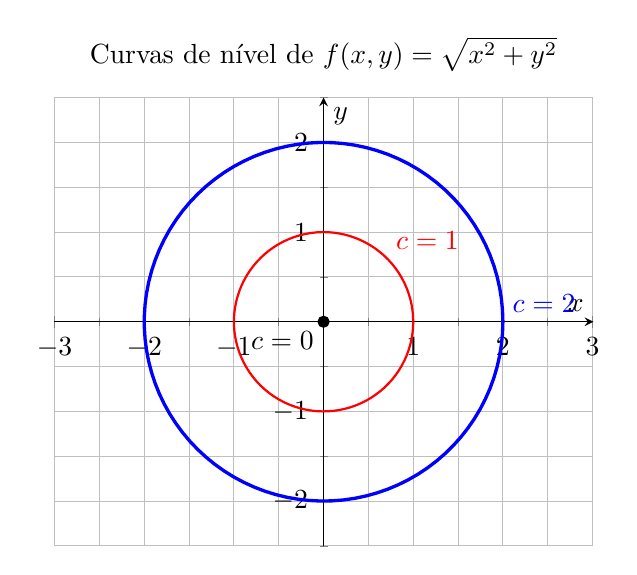
\begin{tikzpicture}
    \begin{axis}[
        axis equal,
        xmin=-2.5, xmax=2.5,
        ymin=-2.5, ymax=2.5,
        axis lines=middle,
        xlabel={$x$},
        ylabel={$y$},
        grid=both,
        minor tick num=1,
        title={Curvas de nível de $f(x,y)=\sqrt{x^2+y^2}$}
    ]

    % círculo c = 2
    \addplot[domain=0:360, samples=100, very thick, color=blue]
    ({2*cos(x)},{2*sin(x)});
    \node[anchor=west, blue] at (axis cs:2,0.2) {$c=2$};

    % círculo c = 1
    \addplot[domain=0:360, samples=100, thick, color=red]
    ({1*cos(x)},{1*sin(x)});
    \node[anchor=south west, red] at (axis cs:0.7,0.7) {$c=1$};

    % ponto c = 0
    \addplot[mark=*, only marks, mark size=2pt, color=black]
    coordinates {(0,0)};
    \node[anchor=north east] at (axis cs:0,0) {$c=0$};

    \end{axis}
\end{tikzpicture}
\caption{Curvas de nível para $c=0, 1, 2$ (Cones).}
\end{figure}

\subsubsection{Plano Tangente}
Seja a função:
\[ f(x,y) = \begin{cases}
  \frac{x^2 - 4y}{x^2 + y^2}, & \quad (x,y) \neq (0,0) \\
  0, & \quad (x,y) = (0,0)
\end{cases} \]
